\documentclass[a4paper, 11pt]{report} %twoside
\title{Invproy\space $\alpha$.zip}
\author{David Davó Laviña}
\date{\today{}}

%%Packages
\usepackage[utf8]{inputenc} %Para saber el encoding del archivo
\usepackage[T1]{fontenc}
%\usepackage[no-math]{fontspec} %Para usar fuentes del sistema
\usepackage{fontspec}

\usepackage{inconsolata}
\usepackage{uarial}
\usepackage{palatino}

\usepackage[xindy, nomain, acronym, acronyms, nonumberlist, nopostdot, toc]{glossaries}
\usepackage{glossary-mcols}
%\usepackage{glossary-custom}

\usepackage[ampersand]{easylist} %Cosas de listas

\usepackage{titlesec}

\usepackage{graphicx} %Para insertar gráficos
\usepackage{float} %PAra posicionar bien los gráficos
\usepackage{unicode-math} %Para símbolos matemagicos
\usepackage[type={CC}, modifier={by-sa}, version={4.0},
lang=spanish]{doclicense} %Muestra la licencia
\usepackage[usenames,svgnames,table]{xcolor} %Para darle color
\usepackage{dirtytalk} %Usado para citar
\usepackage{fvextra}
\usepackage{csquotes} %lo mismo que el anterior pero con estilo
\usepackage[spanish]{babel} %Hace que el idioma de los defaults esté en Español
\usepackage{fancyhdr} %Para poner encabezados y pies de página
%De la bibliografía y las citas.
\usepackage[
backend=biber,
style=ieee
]{biblatex}
\usepackage{tocloft}

\addbibresource{Bibl.bib}
	
\titleformat{\chapter}[display]
    {\color{Black}\normalfont\huge\bfseries}
    {\color{Black}\chaptertitlename\ \thechapter}{20pt}{\Huge}
\titlespacing*{\chapter}{0pt}{-10pt}{10pt}

%Decoraciones y formato del texto
\usepackage[a4paper, left=2.5cm, right=2.5cm, top=3cm, bottom=3cm, headheight=14pt]{geometry}

\usepackage[cache=false]{minted} %Para insertar código

\usepackage{tabularx} %Para hacer tablas muy bonicas
\usepackage{multirow}
\usepackage{array}

\usepackage{caption}%Para insertar cosillas
\usepackage{subcaption}
\usepackage{sidecap}

\usepackage[normalem]{ulem}

\setmainfont{Palatino Linotype}
\setmonofont{Inconsolata}
\setsansfont{Arial}

\setmathrm{Asana-Math.otf}
\setmathsf{Arial}
\setmathtt{Inconsolata}

\fontsize{12}{14}
%Pies de pagina y eso
\pagestyle{fancy}
\fancyhf{}
\makeatletter
\fancyhead[LE, RO]{\@author}
\fancyhead[RE, LO]{\bf\sffamily\color{DarkRed}\@title}
\fancyfoot[LE, RO]{\thepage}
\fancyfoot[C]{\leftmark}

\makeglossaries
\newglossaryentry{Libr}
{
	name=Librería,
	description={En informática, una librería o biblioteca es un conjunto de recursos y fucniones diseñadas para ser usadas por otros programas. Incluyen plantillas, funciones y clases, subrutinas, código escrito, variables predefinidas...},
	plural=librerías,
}
\newglossaryentry{datos}{
	name=Datos,
	description={Secuencia binaria de unos y ceros que contiene información codificada},
	plural=Datos, 
}
\newacronym{gnu}{GNU}{\textit{GNU's Not Unix} (GNU no es Unix)}
\newglossaryentry{Linux}
{
  name=Linux,
  description={is a generic term referring to the family of Unix-like
               computer operating systems that use the Linux kernel},
  plural=Linuces
}
\newglossaryentry{conmutacion de paquetes}{
	name={Conmutación de paquetes},
	description={Método para enviar datos por una red de computadoras. Se divide el paquete en dos partes, una con información de control que leen los nodos para enviar el paquete a su destino y los datos a enviar},
}
\newacronym{osi}{OSI}{\textit{Open Systems Interconnection} (Interconexión de Sistemas Abiertos)}
\newglossaryentry{gls-ISO}{
	name={\textit{International Organization for Standardization}},
	description={Organización Internacional de Normalización. Compuesta de varias organizaciones nacionales se encarga de la creación de estándares internacionales desde 1947.},
}
\newacronym[see={[Glossary:]{gls-ISO}}]{iso}{ISO}{\textit{International Organization for Standardization}\glsadd{gls-ISO}}
\newglossaryentry{capas de abstraccion}{
	name={capas de abstracción},
	description={Método de ocultar detalles de implementación de un set de funcionalidades},
}
\newacronym{IEEE}{IEEE}{Instituto de Ingeniería Eléctrica y Electrónica}
\newglossaryentry{topologia de red}{
	name={topología de red},
	description={Configuración espacial o física de la red. (Ver \ref{topdred} pág.\pageref{topdred})},
	plural={topologías de red},
	see={topologia}
}
\newglossaryentry{topologia}{
	name={topología},
	description={``Rama de las matemáticas que trata especialmente de la continuidad y de otros conceptos más generales originados de ella, como las propiedades de las figuras con independencia de su tamaño o forma." \cite{rae}[Topología]},
	plural={topologías},
}
\newglossaryentry{hardware}{
	name={hardware},
	description={Conjunto de elementos físicos o materiales que constituyen un sistema informático.},
}
\newacronym{MAC}{MAC}{\textit{Media Access Control}, Control de Acceso al Medio}
\newacronym{ADSL}{ADSL}{\textit{Asymmetric Digital Subscriber Line} [Línea de Abonado Digital Asimétrica]}
\newacronym{LAN}{LAN}{\textit{Local Area Network} [Red de Área Local]}
\newacronym{FTTH}{FTTH}{\textit{Fiber To The Home} [Fibra hasta el hogar]}
\newacronym[see={[Glossary:]{gls-FTTx}}]{FTTx}{FTTx}{\textit{Fiber to the X \glsadd{gls-FTTx}}}
\newglossaryentry{gls-FTTx}{
	name={FTTx},
	description={Término que agrupa las distintas configuraciones de acometida de la fibra óptica.},
}
\newglossaryentry{bit}{
	name={bit},
	description={\textit{\textbf{Bi}nary digi\textbf{t}, o dígito binario. Cada dígito del sistema de numeración binario}},
	plural={bits}
}
\newacronym{POP3}{POP3}{\textit{Post Office Protocol}, Protocolo de Oficina Postal}
\newacronym{url}{URL}{\textit{Uniform Resource Identifier}, Identificador de Recursos Uniforme}
\newglossaryentry{cache}{
	name={caché},
	description={Almacenamiento temporal de datos con el objetivo de reducir el retardo, la carga de los servidores y el ancho de banda consumido},
}
\newglossaryentry{programacion imperativa}{
	name={programación imperativa},
	description={Las órdenes del programa cambian el estado de este mismo. Por ejemplo, una variable no tiene por que ser declarada con antelación y su valor es modificable. Es la que usa el código máquina de los ordenadores},
}
\newglossaryentry{botnet}{
	name={botnet},
	description={Grupo de ordenadores coordinados conectados a un maestro mediante un virus. Gracias a este virus se pueden realizar tareas masivas como el envío de SPAM o ataques DDoS},
}
\newglossaryentry{bug}{
	name={bug},
	plural={bugs},
	description={Error en un programa informático.},
}
\newglossaryentry{repositorio}{
	name={repositorio},
	plural={repositorios},
	description={Servidor donde se alojan ficheros o archivos para su descarga},
}
\newglossaryentry{dependencia}{
	plural={dependencias},
	name={dependencia},
	description={De un programa, otro tipo de software necesario para que éste funcione}
}
\newacronym{FSF}{FSF}{\textit{Free Software Foundation}, Fundación del Software Libre}
\newacronym{IDE}{IDE}{Entorno de Desarrollo Integrado, \textit{Integrated Development Enviroment}}
\newacronym{GUI}{GUI}{Interfaz Gráfica de Usuario, \textit{Graphic User Interface})}

%%% Algunas macros
\newcommand{\acr}[1]{\acrshort{#1} (\acrlong{#1})}
\DeclareFontShape{EU1}{Inconsolata(0)}{bx}{n}{<->ssub*Inconsolata(0)/m/n}{}
\usepackage{setspace}
%\onehalfspacing
%\linespread{1.25}
\linespread{1.5}

%Document
\begin{document} %#######################

\makeatletter
\begin{titlepage}{\fontsize{11}{14}
\definecolor{notecolour}{HTML}{CDB380} %TERRA
\newgeometry{a4paper, left=1.2cm, right=1cm, top=3cm, bottom=2cm, headheight=14pt}
\centering
\vspace*{1cm}
{\sffamily\scshape\huge IES Palas Atenea \par}
\vspace{2cm}
{\sffamily\scshape\LARGE Proyecto de Investigación Bachillerato de excelencia:\\
Programación, redes y software libre\par}
\vspace{1.5cm}
{\sffamily\fontsize{42pt}{42pt}\bfseries\color{DarkRed} \@title\par}
{\sffamily\fontsize{24pt}{24pt}\bfseries Un simulador de redes por y para alumnos \par}
{\sffamily\color{DarkRed}\rule{0.5\textwidth}{1pt}\par}
\vspace{.3cm}
{\sffamily\small Adaptación para el \textit{II Encuentro Preuniversitario Jóvenes Investigadores}\par}
\vspace{1.6cm}
{\sffamily\LARGE\itshape \@author\par}
\vfill
{\sffamily\Large Tutor\par
Julio Sánchez Olías}

\vfill

{\sffamily\Large \@date\par}
\pagenumbering{gobble}
\restoregeometry
}
\end{titlepage}
\clearpage

\pagenumbering{Roman}

%\definecolor{chaptercolour}{HTML}{540006}
%\definecolor{sectioncolour}{HTML}{7B1018}
%\definecolor{subsectioncolour}{HTML}{A22F37}
%\definecolor{subsubsectioncolour}{HTML}{CDB380} %TERRA
%%\definecolor{subsubsectioncolour}{HTML}{D46A6A}

\definecolor{chaptercolour}{HTML}{710000}
\definecolor{sectioncolour}{HTML}{8B0000}
\definecolor{subsectioncolour}{HTML}{A20E0E}
\definecolor{subsubsectioncolour}{HTML}{CDB380} %TERRA
%\definecolor{subsubsectioncolour}{HTML}{D46A6A}
%\usemintedstyle{friendly}
\usemintedstyle{borland}

\renewcommand\cftchapfont{\bf\color{chaptercolour}}
\renewcommand\cftchappagefont{\bf\color{chaptercolour}}

\titleformat{\chapter}[display]
%    {\color{chaptercolour}\normalfont\huge\bfseries}
    {\color{chaptercolour}\bfseries}
    {}{0pt}{\huge\thechapter .}
    \titlespacing*{\chapter}{0pt}{-50pt}{10pt}
\titleformat{\section}
	{\color{sectioncolour}\normalfont\Large\bfseries}
	{\color{sectioncolour}\thesection}{1em}{}
\titleformat{\subsection}
	{\color{subsectioncolour}\normalfont\large\bfseries}
	{\color{subsectioncolour}\thesubsection}{1em}{}
\titleformat{\subsubsection}
	{\color{subsubsectioncolour}\normalfont\normalsize\bfseries}
	{\color{subsubsectioncolour}\thesubsubsection}{1em}{}
\renewcommand{\cfttoctitlefont}{\huge\bfseries\color{chaptercolour}}
\renewcommand{\cftloftitlefont}{\huge\bfseries\color{chaptercolour}}

\tableofcontents

\vspace*{1cm}
\listoffigures Todas las imágenes son de autoría propia y siguen la licencia de este documento. \doclicenseName \doclicenseIcon
\newpage{}
\setlength{\parskip}{5pt plus4pt minus3pt}
\setlength{\footskip}{1cm plus4pt minus3pt}

\chapter*{Introducción}
\addcontentsline{toc}{chapter}{Introducción}
En el mundo contemporáneo, ninguna de las innovaciones tecnológicas sería posible sin algo fundamental: las redes; y, más concretamente, redes informáticas. Las redes informáticas han hecho posible, desde su nacimiento, la comunicación de grandes sumas de datos a velocidades casi instantáneas entre sitios distantes. Al principio esta tecnología era usada entre universidades, acelerando el proceso de investigación al coordinarse unas universidades con otras mucho más rápidamente. 

Más tarde, se extendió el uso de esta tecnología del uso militar y científico a todas las empresas y hogares, comenzando así una revolución tecnológica que aún no se ha conseguido parar. Con acceso instantáneo a cultura, entretenimiento, conocimiento, información y más de dos mil exabytes de ancho de banda\footnote{Datos a Mayo de 2015. Fuente: Cisco--\cite{Cisco}} viajando por la red, se ha convertido en una herramienta de uso por la humanidad imprescindible para cualquier actividad.

La tecnología del mundo contemporáneo no habría sido posible, en parte, también gracias al software libre y al desarrollo colaborativo, pues ha permitido el desarrollo de sistemas operativos como GNU/Linux de la \textit{Free Software Foundation} (Usado actualmente por el 90\% de los servidores de red) o CUPS, el software para servidores de administración de impresoras más completo y competente usado en la mayoría de oficinas.

Son dos cosas muy importantes, que apenas son enseñadas en las clases de la ESO y Bachillerato, por eso he creado InvProy, un pequeño simulador de redes con la ambición de enseñar tanto de redes como de programación. Podrán experimentar, de una forma sencilla y muy visual como funciona una red y cómo se comportan los distintos protocolos. También, al ser software libre, los alumnos podrán aprender sobre programación al observar el código y tener la licencia para modificarlo y colaborar en el desarrollo del programa. Aunque el programa este aún en fase Alpha (fase de desarrollo), ya tiene la base para que sea muy sencillo añadir más protocolos, funcionalidades o dispositivos de red. A día de hoy tiene como dispositivos los ordenadores, conmutadores y concentradores. En cuanto a paquetes de red, permite enviar un Ping, usando los protocolos ICMP, IPv4 y Ethernet.

\newpage
%LA GRANA ANTIGUA
%\definecolor{chaptercolour}{HTML}{550000}
%\definecolor{sectioncolour}{HTML}{801515}
%\definecolor{subsectioncolour}{HTML}{AA3939}
%\definecolor{subsubsectioncolour}{HTML}{CDB380} %TERRA
%%\definecolor{subsubsectioncolour}{HTML}{D46A6A}

\setcounter{chapter}{0}    
\chapter{Programación y software libre}
\pagenumbering{arabic}

\subsection*{Propuesta}
El objetivo de este proyecto es el desarrollo abierto  y colaborativo a largo plazo de un software programado en Python de código libre con el que los alumnos puedan aprender tanto sobre redes como de programación. Debe soportar los protocolos más utilizados en la actualidad y permitir una gran personalización por los usuarios. Además debe ser compatible con los sistemas operativos Ubuntu, MaX y Windows, y ser de fácil instalación para el alumnado. Debe ser intuitivo y fácil de usar e incluir una gran documentación.

\section{Software Libre}
Según la Free Software Foundation
\say{«Software libre» es el software que respeta la libertad de los usuarios y la comunidad. A grandes rasgos, significa que los usuarios tienen la libertad de ejecutar, copiar, distribuir, estudiar, modificar y mejorar el software. Es decir, el «software libre» es una cuestión de libertad, no de precio. Para entender el concepto, piense en «libre» como en «libre expresión», no como en «barra libre». En inglés a veces decimos «libre software», en lugar de «free software», para mostrar que no queremos decir que es gratuito.}
-- R. Stallman \cite{FSF-Ph}

No debemos confundir `Software Libre' con `Código abierto', ya que, aunque el código pueda ser leído por todo el mundo no significa que el resto de personas tengan licencia para redistribuir y/o editar el código. Software libre es el que cumple: \cite{FSF-talk1, FSF-talk2}
\begin{easylist}[itemize]
\ListProperties(Style*=$\bullet$ , Style2*=--)
& \textbf{Libertad 0:} La libertad de ejecutar el programa cuando quieras, para cualquier propósito.
& \textbf{Libertad 1:} La libertad de estudiar cómo el programa funciona, y la posibilidad de cambiarlo para que se ejecute como tú deseas. (Acceso al código del programa).
& \textbf{Libertad 2:} La libertad de redistribuir las copias para ayudar a tus colegas.
& \textbf{Libertad 3:} La libertad de distribuir copias de tu versión modificada a otras personas.
\end{easylist}

Una de las grandes ventajas del software libre, aparece en la educación. Es muy útil para aprender ya que, si un alumno tiene curiosidad sobre el programa que está usando, puede consultar el código fuente en internet. Además, al ser licencias gratuitas, se puede destinar ese presupuesto a otras áreas como el hardware o el profesorado. También es útil en el desarrollo, pues cualquier programador puede solucionar un error que afecta a todos los usuarios.

\newpage

%\definecolor{chaptercolour}{HTML}{051C38}
%\definecolor{sectioncolour}{HTML}{143153}
%\definecolor{subsectioncolour}{HTML}{4B688B}
%%\definecolor{subsubsectioncolour}{HTML}{CDB380} %TERRA
%\definecolor{subsubsectioncolour}{HTML}{748BA7}
\chapter{Redes Informáticas}

\section{Capas de Red/Modelo OSI}
El modelo \acrshort{osi} es un modelo de referencia para redes basado en \gls{capas de abstraccion}.
Su objetivo es conseguir la interoperabilidad entre sistemas haciendo uso de los protocolos estandarizados. Fue creado en 1980 por la Organización Internacional de Estandarización (\acrshort{iso}). No es considerado una arquitectura de red porque los protocolos no forman parte del modelo, sino que son entidades de distintas normativas internacionales.
\definecolor{odd}{HTML}{FFFFFF}
%\definecolor{even}{HTML}{E0E0E0}
\definecolor{even}{HTML}{FCE4EC}
\definecolor{header}{HTML}{EF9A9A}
%\definecolor{header}{HTML}{F48FB1}
\vspace*{20pt}

\rowcolors{1}{header}{header}
\rowcolors{2}{odd}{even}
\renewcommand{\arraystretch}{1} %Antes 1.1
\noindent\linespread{1}
\begin{tabularx}{\linewidth}{ | c >{\small}c >{\small}X >{\small}c | }
	\rowcolor{header} \hline
	\textbf{Capa} & \textbf{PDU\footnote{\textit{Protocol Data Unit} o Unidad de Datos de Protocolo.}} & \textbf{Función} & \textbf{Ejemplos} \\ \hline
	1. Física & Bit & Transmisión y recepción de bits físicos sobre un medio físico (topología de red) & 	 RJ45, IEEE 802.11, etc. \\
	\label{osi}
	2. Data Link & Frame & Transmisión segura de \textit{frames} entre dos nodos conectados por una capa física. & Ethernet, 802.11, etc...\\
	3. Red & Paquete & Estructurar y administrar una red multinodo. Incluye enrutamiento, control de tráfico, y asignación de direcciones & IPv4, IPv6, ICMP... \\
	4. Transporte & \begin{tabular}[t]{@{}c@{}}Datagrama(UDP)\\Segmento(TCP)  \end{tabular} &
	Transmisión de segmentos de datos entre los puntos de una red, incluyendo ACK & TCP, UDP...\\
	5. Sesión & Datos & Administración de sesiones de comunicación, como intercambio continúo de información entre dos nodos. & SSH, RPC, PAP...\\ 
	6. Presentación & Datos & Translación de datos entre un servicio de red y una aplicación. Incluye comprensión, encriptación/decriptación, y codificación de carácteres. & MIME, TLS \\
	7. Aplicación & Datos & APIs de alto nivel, incluyendo recursos compartidos y acceso remoto de archivos & HTTP, FTP, SMTP... \\ \hline
\end{tabularx}
\newpage

\section{Paquetes de red}
Son cada serie de bits en los que se divide la información enviada por una red. \\ Según el modelo OSI, un paquete es estrictamente el PDU de la capa de red. El paquete de red se encuentra encapsulado en la capa anterior del modelo OSI. Por ejemplo, en éstandares de comunicación TCP/IP, un segmento TCP puede ser llevado por varios paquetes IP transportados por varios frames de Ethernet. Es parecido a las unidades lingüísticas. \\Está formado por varios protocolos y en él se distinguen tres partes:
\begin{description}
\item \textbf{Header} o cabecera: Datos e información sobre el paquete. (Dirección IP, MAC, etc)
\item \textbf{Payload} o carga: Los datos que se quieren transferir.
\item \textbf{Trailer} o cola: En ocasiones es inexistente (como en UDP) pero suele ser un código de comprobación de errores.
\end{description}

\vspace{1cm}
\begin{figure}[H]
\noindent
\centering
\includegraphics[width=\textwidth]{Resources/Encapsulación_OSI.pdf}
\caption{Encapsulación de red. El Datagrama IP es lo considerado 'Paquete de red'}
\end{figure}
\vspace{\fill}
\newpage

\section{Protocolos}
Un protocolo de comunicación es un conjunto de reglas para intercambiar información entre enlaces de red. En una pila de protocolos, cada protocolo cubre los servicios del protocolo de la capa anterior. Por ejemplo, un e-mail se envía mediante el protocolo \acr{POP3} en la capa de Aplicación, sobre TCP en la capa de transporte, sobre IP en la capa de Red, sobre Ethernet para la capa \textit{Data Link}, que está formado por bits. Para entenderlo mejor, es como la gramática de la lengua. Un sustantivo forma parte de un sintagma nominal, que forma parte de un sujeto, que a su vez forma parte de una oración. Siendo las ondas sonoras producidas la capa física y fonemas los bits.
\begin{figure}[H]
\noindent
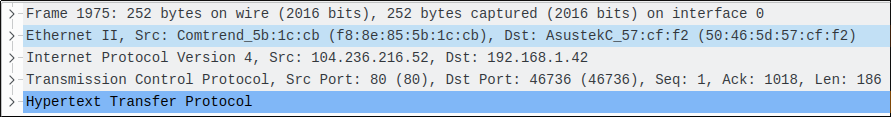
\includegraphics[width=\textwidth]{Resources/Wireshark01.png}
\caption[Captura de pantalla de Wireshark]{Captura de pantalla de Wireshark (Véase \ref{wireshark}, pg. \pageref{wireshark}) en la que se muestran los protocolos que forman un paquete de red HTTP.}
\end{figure}

\subsection{Familia de protocolos de internet}
También conocido como \textit{Internet Protocol Suite}, y más conocido como TCP/IP, es el fundamento de las redes informáticas. Se trata de un conjunto de más de 100 protocolos que permiten la conexión de ordenadores tanto en Internet como en LAN, incluyendo protocolos de las aplicaciones más usadas.

\setcounter{secnumdepth}{5}
\subsubsection{Aplicación}
Es la capa en la que se envían los datos a otras aplicaciones en otro ordenador o en el mismo. Las aplicaciones hacen uso de las capas inferiores para asegurarse que los datos lleguen a su destino. Algunos de los protocolos más usados son:
\begin{itemize}
\item \textbf{HTTP} \textit{Hypertex Transfer Protocol:} Protocolo de Transferencia de Hipertexto. Es el protocolo base de la World Wide Web. Se trata de texto estructurado que usa hiperenlaces entre nodos que también contienen texto. El cliente, al entrar en una \acr{url} a través de el agente de usuario (navegador) envía al servidor una petición de la página web, mediante HTTP. El servidor, envía como respuesta un documento HTML u otro recurso.
\item \textbf{DNS} \textit{Domain Name System:} Sistema de Nombres de Dominio. Un servidor DNS almacena una base de datos distribuida y jerárquica con información sobre el nombre del dominio y la dirección IP a la que está vinculada. Al intentar conectar a  \texttt{ddavo.me}, el cliente pregunta al servidor cual es la dirección IP asociada a esa dirección, y se conecta a tal IP, en este caso 37.152.88.18. Para evitar tener que consultar continuamente con el servidor, se almacenan en una \gls{cache} en el cliente.
\item \textbf{DHCP} \textit{Dynamic Host Configuration Protocol}: Protocolo de configuración dinámica del host. Este protocolo es controlado por un servidor DHCP que envía parámetros de configuración automática a los clientes. El ejemplo más común es el de cualquier Router doméstico, que asigna automáticamente a cada dispositivo una dirección IP diferente, pero dejando un rango en el que se pueden establecer IP's estáticas.
\end{itemize}
\subsubsection{Transporte}
Se encapsulan los datos de aplicación en un segmento o datagrama, dependiendo si el protocolo usado es TCP o UDP. Se encarga de transportar los datos por una red independientemente de la topología física.
\begin{itemize}
\item \textbf{TCP} \textit{Transmission Control Protocol:} Protocolo de Control de Transmisión. Se aplica a los paquetes para administrarles un orden y un sistema de comprobación de errores. Con todas las funcionalidades, ocupa bastante espacio, lo que aumenta la latencia, aunque es más fiable para el envío de la mayoría de los datos.
\item \textbf{UDP} \textit{User Datagram Protocol:} Es un protocolo muy minimalista. A diferencia del TCP, no garantiza que los paquetes lleguen, o lleguen en orden, o protección ante duplicados. Reduce mucho la latencia ya que no usa \textit{handshaking}. Por ello es usado por ejemplo para \textit{streamings} de televisión o videollamadas.
\end{itemize}
\subsubsection{Red}
El objetivo es que los datos lleguen del origen al destino, aún cuando no están conectados directamente. Los enrutadores o \textit{routers} son los dispositivos que cumplen esta función.
\begin{itemize}
\item \textbf{IP} \textit{Internet Protocol}: Protocolo de Internet. Envía datagramas o paquetes de red a través de redes. Tiene una función de enrutamiento que es la que permite la interconexión de redes, y la existencia de Internet. Es un protocolo que encapsula el paquete definiendo en el \textit{header} (cabecera) las direcciones IP del servidor y el cliente, o remitente y destinatario. La versión usada actualmente es IPv4 desarrollado en 1981, pero poco a poco se va abriendo paso la versión IPv6. La mayor diferencia es que la versión cuatro cuenta con direcciones de 32 bits lo que permite tan sólo unos 4.3 millardos ($\mathsf{2^{32}}$) de direcciones, mientras que la versión 6 tiene direcciones de 128 bits, lo que permite más de 340 sextillones ($\mathsf{2^{128}}$) de direcciones
\item \textbf{ICMP} \textit{Internect Control Message Protocol}: Es un protocolo que no es usado por aplicaciones de usuario (a excepción de herramientas de diagnóstico como ping o traceroute). Lo usan los dispositivos de red, como los routers, para enviar notificaciones o mensajes de error indicando que un servicio no está disponible.
\end{itemize}
\subsubsection{Link}
Capa encargada del acceso al medio físico de la red. También cumple otras funciones como incluir una comprobación de errores e identificar cada dispositivo de forma única.
\begin{itemize}
\item \textbf{ARP} \textit{Address Resolution Protocol:} Protocolo de resolución de direcciones. Es un protocolo que convierte direcciones de la capa de Red a la capa de Enlace (dir. IP a dir. MAC). El dispositivo, al conectarse una red, envía un \textit{frame} ARP con su dirección MAC y su IP, para que los demás dispositivos de la red lo almacenen en su memoria y poder usar ambas direcciones al enviar un paquete.
\item \textbf{MAC} \textit{Media access control}: Control de acceso al medio. Es un conjunto de protocolos (Como Ethernet o IEEE 802.11 [WiFi]) encargados de asignar el medio físico de la red. Evita colisiones entre paquetes asegurándose de que el medio está libre y evitando así la transmisión simultánea.
\end{itemize}

\newcommand{\function}[1]{\texttt{\color{Orange}#1}}
\newcommand{\class}[1]{\texttt{\color{DarkRed}#1}}
\chapter{El simulador de redes}
La parte práctica del Proyecto de Investigación, el simulador de redes de nombre \textit{InvProy}, ha sido la parte más extensa del proyecto, que más tiempo, esfuerzo y recursos ha ocupado. Se podría decir que el proyecto entero es la parte práctica. Como curiosidad, el nombre de \textit{InvProy} viene del acrónimo formado mediante la permutación de las palabras ``Proyecto de Investigación", quedando \textit{``Investigación \sout{de} Proyecto"} y de ahí \textit{InvProy}.

\section{Herramientas usadas en la creación del software}
Todo el software que se ha usado para la creación de este programa, es software libre, debido a las ventajas citadas anteriormente. A continuación, se listan las herramientas que se han usado para la creación tanto del programa como de este documento.

\subsection{GNU/Linux}
También llamado incorrectamente sólo Linux, es una manera de llamar al Sistema Operativo (OS) combinación del kernel Linux (Basado en Unix) y el OS \acrshort{gnu} (Acrónimo recursivo \textit{GNU's Not Unix}, o GNU no es Unix). Es el gran ejemplo por excelencia del Software Libre. Es el sistema operativo más utilizado, pues es usado en la mayoría de los servidores, y además, otros sistemas operativos como Android están basados en éste. Puedes instalar Linux desde el código fuente o instalar distribuciones o \textit{distros} (conjunto de software preconfigurado y compilado que contiene GNU, Linux y otros paquetes). Se han usado Arch Linux, Ubuntu 16 y MaX 8.

\subsubsection{Distros}
Son las distintas distribuciones de software de GNU/Linux. Es decir, un conjunto de software preconfigurado y compilado formado por el Sistema Operativo GNU, el kernel de Linux y otros tantos paquetes, dependiendo de los usuarios a los que esté dirigida la distribución. Pueden crearse con el soporte de una empresa; como Ubuntu (Canonical Ltd.), openSUSE (Novell) o Fedora (Red Hat); y otras mantenidas por comunidades como Debian, Gentoo o Arch Linux.

\subsection{Git y Github}
Git es un software diseñado por Linus Torvalds con el que se puede crear un Sistema de
Control de Versiones (VCS). Este programa te permite
de forma sencilla volver a una versión o \textit{commit} anterior del programa, así
como enviarlas a un \gls{repositorio} remoto e incluso publicarlas en línea. Su punto fuerte
son las \textit{branches} o ``ramificaciones" del código, haciendo que la rama
\textit{master} (principal) siempre sea funcional. Para ello creamos una nueva rama para cada nueva funcionalidad del programa. La implementación del nuevo código a otra rama se denomina \textit{merge}. Otra de las funcionalidades que implementa es \texttt{clone}, que te permite descargar un proyecto si tienes la URL del \gls{repositorio} git.
\begin{figure}[H]
\noindent
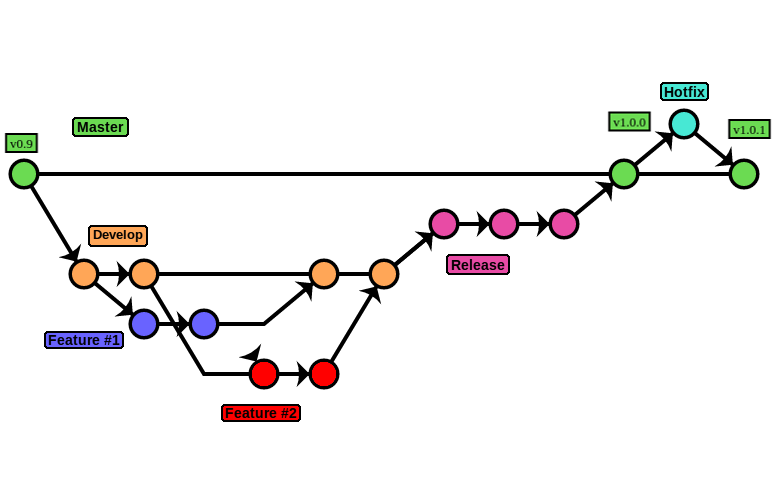
\includegraphics[width=0.9\textwidth]{Resources/Gitflow.png}
\caption{\textit{Gitflow} o flujo de trabajo de Git}
\end{figure}

GitHub es una plataforma de desarrollo colaborativo que te permite alojar tus repositorios Git. Su uso es gratuito si el código almacenado es público. Además, te permite tener una wiki y una página web para tu proyecto, junto a otras funciones.
Una de sus funciones estrella es la visualización online del repositorio, con la que cualquier persona tiene acceso al código y los archivos antes de descargarlos. Otra función útil es el apartado de \textit{Issues}, en el que los usuarios de tu código pueden reportar los bugs del programa o aportar nuevas ideas en forma de "foro".
Tanto el programa como este documento están disponibles en GitHub en los siguientes enlaces. \url{https://github.com/daviddavo/InvProy} y \url{https://github.com/daviddavo/InvProy-tex}

\subsection{LaTeX}
\LaTeX\space o, en texto plano, LaTeX, pronunciado con la letra griega 
Ji ($\Chi$), es un software libre orientado a la creación de textos escritos comparable a la calidad tipográfica de las editoriales. Mediante la importación de paquetes y comandos o macros se puede dar formato al texto al igual que con cualquier otro editor, exportándolo posteriormente a PostScript o PDF. Está orientado a documentos técnicos y científicos por su facilidad a la hora de incluir fórmulas o código e importar paquetes que cumplan las necesidades de los usuarios. No es un procesador de textos, pues está más enfocado en el contenido del documento que en la apariencia de éste.
El código del documento puede ser editado con cualquier editor de texto plano como \textit{nano} o \textit{emacs}, aunque he usado una \acrshort{IDE} llamada \textbf{texmaker}.

\subsection{Python}
\label{python}
Es un lenguaje de programación interpretado (sólo se traduce  el programa a código máquina cuando se debe ejecutar esa parte del código, por lo que no hace falta compilarlo) que destaca porque sus programas poseen una sintaxis más legible que la de el resto de lenguajes. Soporta tanto \gls{programacion imperativa} como programación orientada a objetos. Usa variables dinámicas, es multiplataforma, y, además, es de código abierto, lo que permite distribuir el programa en Windows al distribuir los binarios de Python junto a él. En este proyecto, la versión de Python utilizada es la 3.4 en adelante.

\subsection{Gtk+}
Es un conjunto de bibliotecas o \glspl{Libr} (conjunto de funciones y clases ya definidas preparadas para el uso de los programadores) desarrollado por la GNOME foundation destinado a la creación de Interfaces Gráficas de Usuario (\acrshort{GUI}), también, al igual que Linux forma parte del proyecto GNU.

Al utilizar este conjunto de librerías, se ha conseguido que sólo sea necesario descargar una dependencia del programa, que además suele venir instalada en la mayoria de distros de Linux. Por ejemplo en una instalación limpia de Ubuntu 16 (sin descargar paquetes adicionales) el programa funciona perfectamente. Para usarlo en Python se ha tenido que importar la libreria de PyGtk, que también suele venir incluida en la distribución.

\subsection{Wireshark}
\label{wireshark}
Wireshark es un \textit{packet sniffer} o analizador de paquetes; te muestra los paquetes de red reales enviados y recibidos por una tarjeta de red, lo que facilita la creación del simulador de redes. También te separa las distintas partes de la encapsulación del paquete y además te permite buscar entre los paquetes de red añadidos y recibidos, pudiendo añadir filtros de búsqueda para los distintos campos del paquete y para las distintas capas.

\section{Instalación}
\subsection{Ubuntu / Debian}
En caso de no estar en los repositorios, hay que hacerlo manualmente. Descarga el paquete de \url{https://github.com/daviddavo/InvProy/releases/latest}. Una vez descargado, abre una terminal donde se haya descargado el paquete e instálelo.
\begin{minted}{bash}
~ $ cd Descargas
Descargas $ sudo dpkg -i invproy*.deb
\end{minted}

\section{Uso del programa}
Esta guía ha sido creada usando la versión v0.2.4-alpha, por lo que en algunos apartados pueden haberse realizado cambios en versiones posteriores.

El programa está siendo diseñado para tener una mayor facilidad de uso, pensando en una interfaz intuitiva y simple que pueda ser utilizada sin la necesidad de ningún apoyo externo al programa (instrucciones, documentación, tutor). Para ello, en la versión v0.4 será añadido un asistente o `tutorial' que guíe a los alumnos la primera vez que se acceda al programa; además de añadir más información, dentro de la interfaz, sobre redes.

A continuación, se incluye una captura de pantalla de la interfaz de InvProy Alpha, explicando el funcionamiento de los distintos botones de la interfaz.

\begin{figure}[H]
\noindent\centering
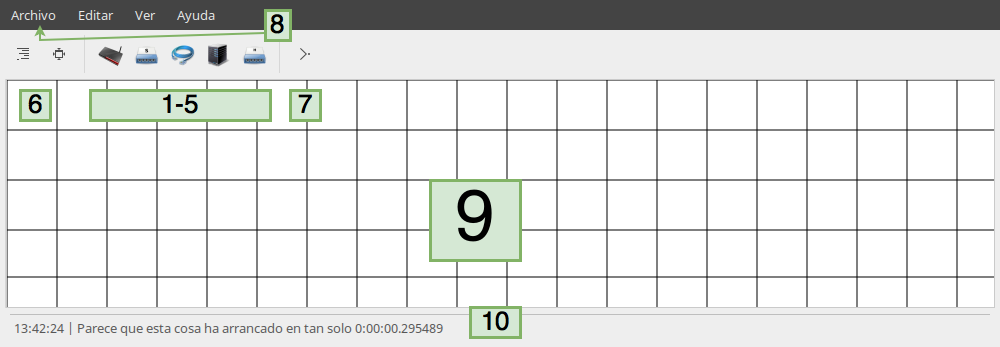
\includegraphics[width=\textwidth]{Resources/Screenshots/2016-09-07-134612_1000x700_scrot.png}
\caption[Interfaz de InvProy Alpha]{Interfaz de InvProy Alpha. Al usar Gtk+, los temas se pueden cambiar, así que la apariencia del programa puede ser distinta dependiendo del tema de escritorio que estés usando.}
\end{figure}
\newenvironment{mydescr}
{ \begin{enumerate}
    \setlength{\itemsep}{0pt}
    \setlength{\parskip}{0pt}
    \setlength{\parsep}{0pt}     }
{ \end{enumerate}                  } 
\begin{mydescr}
\item [1-5.] También se puede activar con las letras Q, W, E, R, T; respectivamente. Los botones, te permiten (de izquierda a derecha): colocar un router, colocar un switch, conectar dos objetos, colocar un ordenador y colocar un hub. Para ello primero haces click en el botón y luego haces click en el lugar donde quieras colocar el objeto. En el caso de los cables debes hacer dos clicks, uno en cada objeto a conectar. 
\item [6.] Abre el menú de ``Información de dispositivos", que proporciona información como la dirección IP y MAC, el nombre, o los dispositivos a los que está conectado. (Ver figura \ref{dispinfo}
\item [7.] Te permite enviar un ping de un ordenador a otro (El botón funciona a partir de v0.3).
\item [8.] Abre el menú de archivo, en el que puedes cargar un archivo, crear uno nuevo, guardarlo, y cerrar el programa.
\item [9.] Es la ventana donde puedes colocar los objetos. Puedes moverte a través de ella y en el menú de `Ver' puedes cambiar el que se vea la rejilla de fondo.
\item [10.] Aquí se encuentra una barra con información sobre el funcionamiento actual del programa.
\end{mydescr}
\begin{figure}[H]
\centering
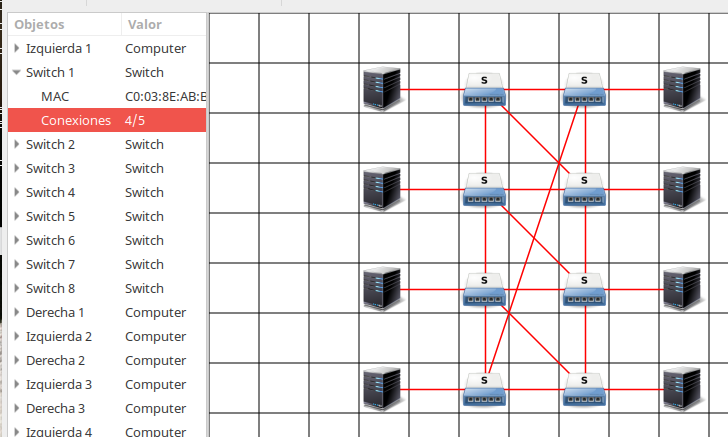
\includegraphics[width=0.9\textwidth]{Resources/Screenshots/2016-09-07-140130_728x437_scrot.png}
\caption[Menú de Información de Dispositivos]{Menú de \textbf{Información de Dispositivos} junto a una red de topología de malla \label{dispinfo}}
\end{figure}
Para incluir un objeto en la rejilla, se hace click en el icono del objeto y luego  en el lugar donde se quiera poner. Cuando tenemos dos objetos podemos conectarlos si hacemos click primero en el icono del cable, luego en un objeto y después en otro.

\section{Funcionamiento del programa}
Se ha creado haciendo uso de todas las herramientas anteriormente mencionadas.

El programa posee distintas clases. Se pueden diferenciar en cuatro tipos: Clases de Interfaz (\class{MainClase}, \class{w\char`_changethings}...), 
Clases de Dispositivos (\class{ObjetoBase, Switch, Computador}), Clases de Red (\class{packet}, \class{frame}) y clases de apoyo (\class{MAC}, \class{IP}, \class{Port}, \class{Cable}).

Todas las clases poseen, como mínimo, una función llamada \function{\char`_\char`_init\char`_\char`_}, que es la encargada de crear el objeto y establecer las variables más importantes (Coordenadas, variables vacías, dirección MAC...).

%\newpage
\subsection{Main.py}
Es el archivo principal del programa. Contiene las funciones más importantes, además de las clases para crear los objetos. Primero trata de importar los módulos necesarios, comprobando uno a uno si están instalados, y advirtiendo al usuario en el caso de que no estén instalados.

\subsubsection{MainClase}
Es la clase principal de la interfaz del programa. Se encarga de administrar la ventana principal de la interfaz.

Posee varias funciones como \function{on\char`_key\char`_press\char`_event} y \function{on\char`_key\char`_release\char`_event} (\texttt{370:416}), que actúan cada vez que se pulsa una tecla y se encargan de hacer las acciones necesarias para esa tecla (o combinación de teclas). Otra función importante es \function{toolbutton\char`_clicked}, que se acciona cada vez que se pulsa un botón (de arriba) y se encarga de comunicarlo a la rejilla.

También contiene una subclase, llamada \class{ObjLst} (\texttt{263:332\footnote{Notación para escribir la ubicación del código. Línea inicial:Línea final@Archivo. Si se omite el nombre de archivo, es porque ha sido anteriormente mencionado.}}), encargada de la lista de objetos de la parte izquierda de la interfaz.

\newpage

\subsubsection{Grid}
Es la clase de la rejilla, se desarrolla de la línea 498 hasta la 677. Tiene varias `capas', una para los cables, otra para el fondo, otra para los dispositivos... Así, en el caso de que dos elementos se solapen, los dispositivos siempre permanecerán al frente del fondo y los cables. El fondo se hace creando una línea horizontal cada \texttt{sq} píxeles, y otras tantas verticales del mismo modo, siendo \texttt{sq} el parámetro \texttt{viewport-sqres} del archivo \texttt{Config.ini}.

\begin{description}
\item \function{clicked\char`_on\char`_grid}: \texttt{578:639} Función que se encarga de realizar distintas acciones dependiendo de dónde se haya hecho click dentro de la rejilla. Para ello, primero debe comprobar si ahí hay o no un objeto, y una vez lo ha comprobado, comprobar si uno de los botones para colocar un objeto ha sido pulsado.
\item \function{gridparser} \texttt{641:651}: Es una función muy sencilla. Te convierte coordenadas de la rejilla, a coordenadas en píxeles (usadas por Gtk).
\item \function{resizetogrid} \texttt{653:657}: Otra función sencilla. Dada una imagen, la convierte al tamaño de un cuadrado de la rejilla.
\item \function{searchforobject} \texttt{659:672}: Encargada de comprobar si, dadas unas coordenadas, hay un objeto en estas.
\item \function{moveto} \texttt{563:576}: Te mueve una imagen dada a unas coordenadas dadas. En el caso de que de que no esté en la rejilla, crea la imagen, y en el caso de que ya esté en ella, la mueve al lugar designado.
\end{description}

\newpage
\subsubsection{ObjetoBase}
En Python, existe la herencia de clases. Esto quiere decir que una clase puede heredar las funciones y los atributos de otra, en forma de cascada. La clase principal de la que heredan el resto de dispositivos de red es \class{ObjetoBase}. Algunas de sus funciones son estas:

\begin{itemize}
\item \function{compcon}: Es una función que poseen todos los dispositivos de red, que dado un objeto \class{Computador}, retorna todos los ordenadores que están conectados a la misma red. Se encuentra en \texttt{822:864}. Está formada por una lista que contendrá los ordenadores conectados y una función llamada subcompcon (\texttt{827:847}), que comprueba las conexiones del objeto, añadiendo la conexión a la lista si es un ordenador. En el caso de que sea un conmutador o un concentrador, llama a la función \texttt{subcompcon} con ese objeto como argumento, por lo que comprueba las conexiones de ese objeto y las añade a la lista del primero, entrando en un bucle hasta que ha comprobado toda la red. La función es usada por el programa cuando es necesario comprobar si dos ordenadores están conectados, por ejemplo. (Ver figura \ref{fig:compcon})
\item \function{load}: \texttt{877:896} Al cargar un objeto de un archivo, hay determinadas propiedades del objeto que deben ser establecidas de cero, y determinadas funciones que deben ser llamadas, para ello existe esta función.
\item \function{update}: Esta función, bastante importante se encarga de actualizar la información del objeto en la interfaz de usuario. Es llamada cada vez que se produce un cambio en el objeto; como al conectarlo, editar el nombre, o desconectarlo de otros objetos.
\item \function{connect}: \texttt{898:941} Esta función se encarga de establecer las conexiones entre dos objetos.
\item \function{disconnect}: \texttt{942:989}. Realiza lo contrario de \function{connect}, desconecta un objeto de otro. O un objeto de todos a los que está conectado.
\item \function{packet\char`_received}: Esta es la función por defecto que se ejecuta cuando un dispositivo ha recibido un paquete. Todos los dispositivos de red tienen una función diferente que sobreescribe a esta (pues no es el mismo comportamiento el de un conmutador que el de un ordenador).
\end{itemize}

\newpage

\thispagestyle{empty}
\begin{figure}
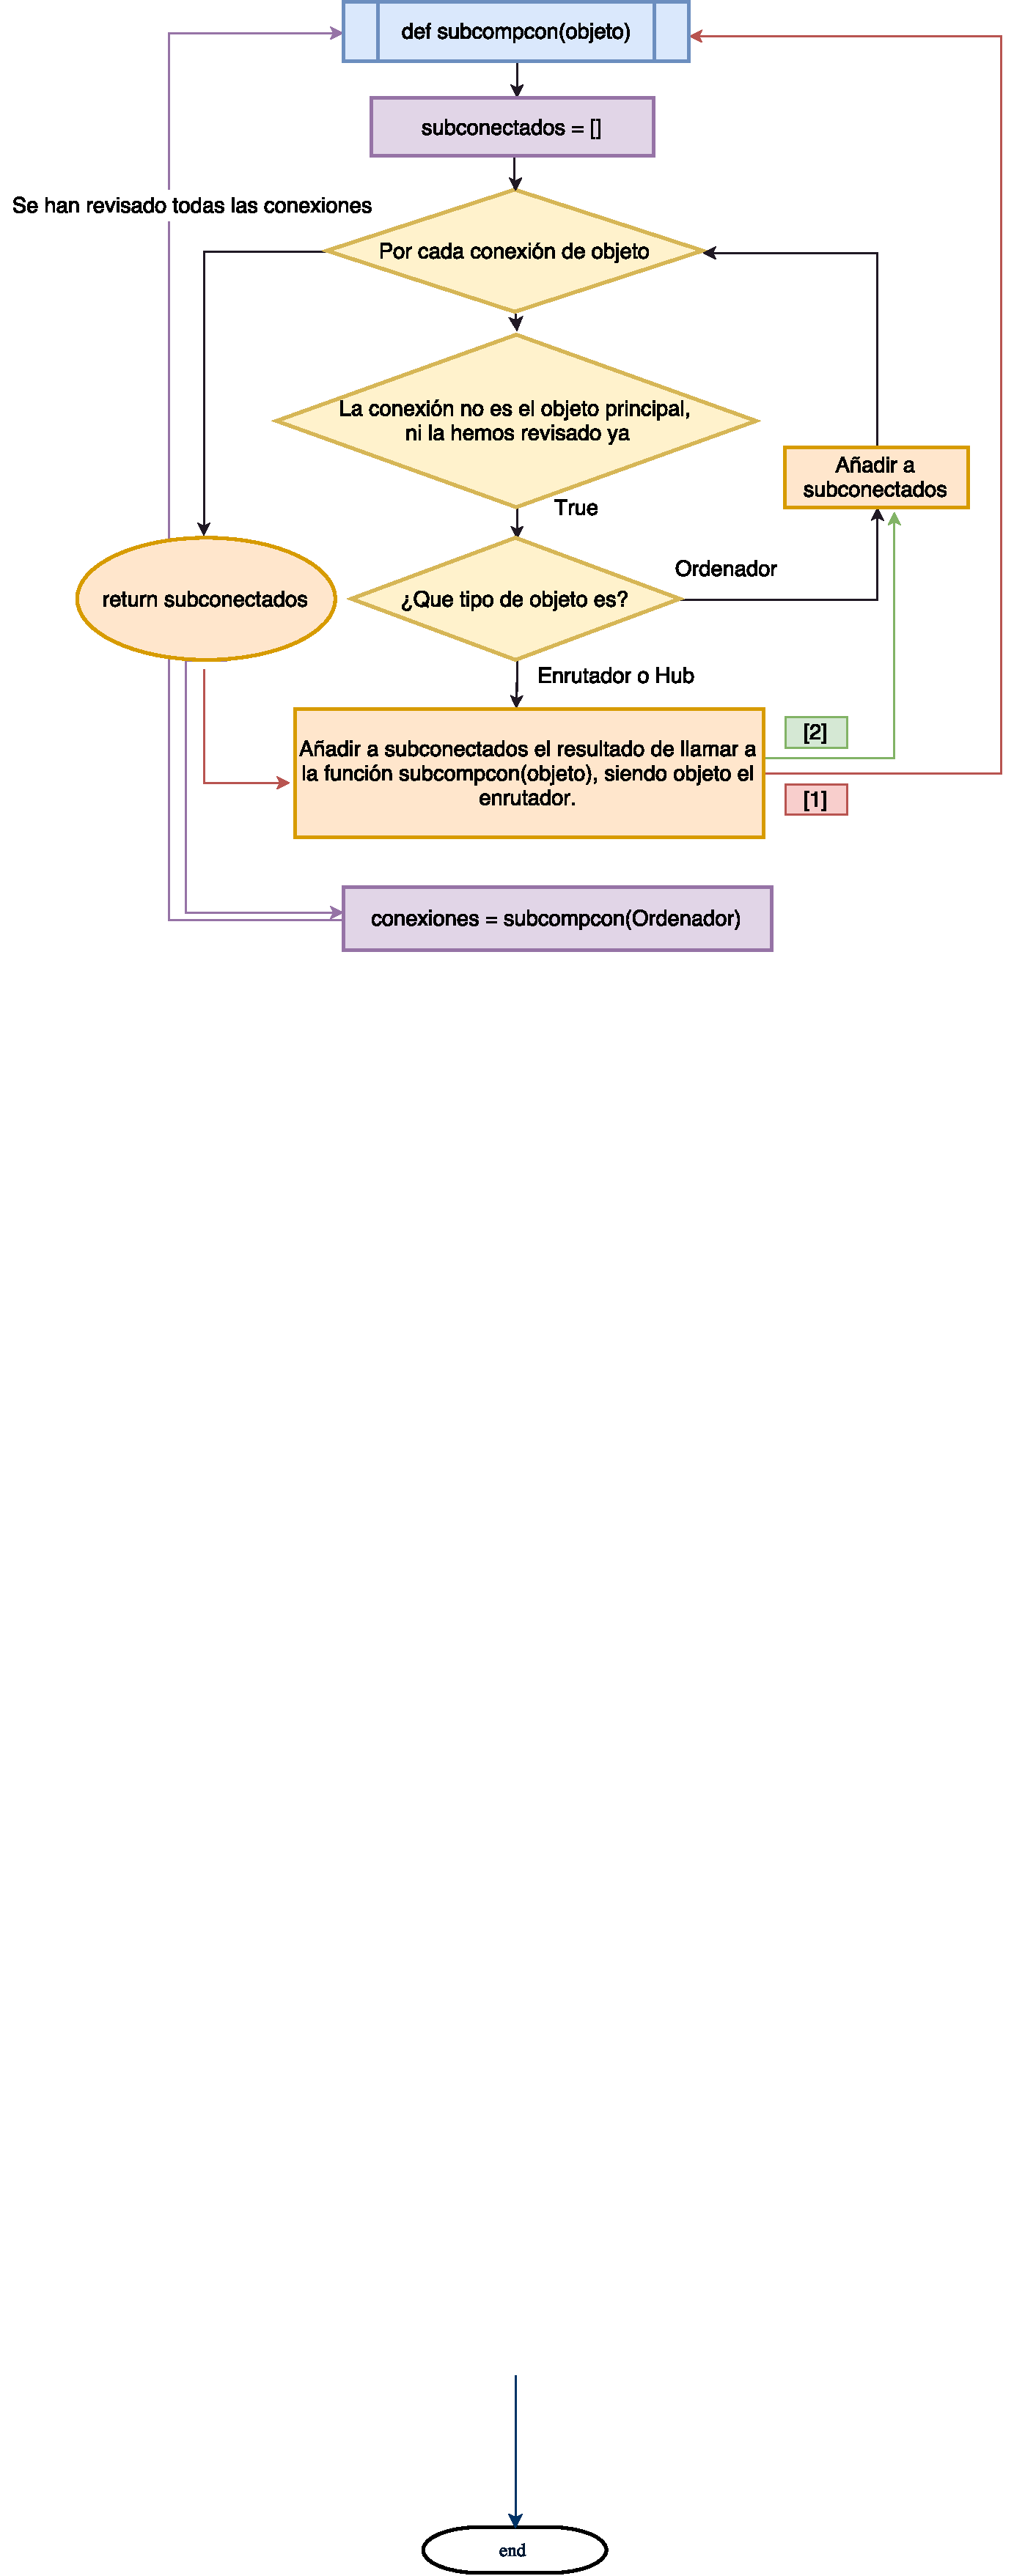
\includegraphics[width=\textwidth]{Resources/Diagramas/Compcon.pdf}

\vspace*{1cm}
\caption[Diagrama de flujo de la función \texttt{compcon}]{\label{fig:compcon}
Diagrama de flujo del funcionamiento de la función \function{compcon}.
}
\end{figure}

\clearpage

%\newpage
%\vspace{\fill}
%\begin{figure}[H]
%\centering
%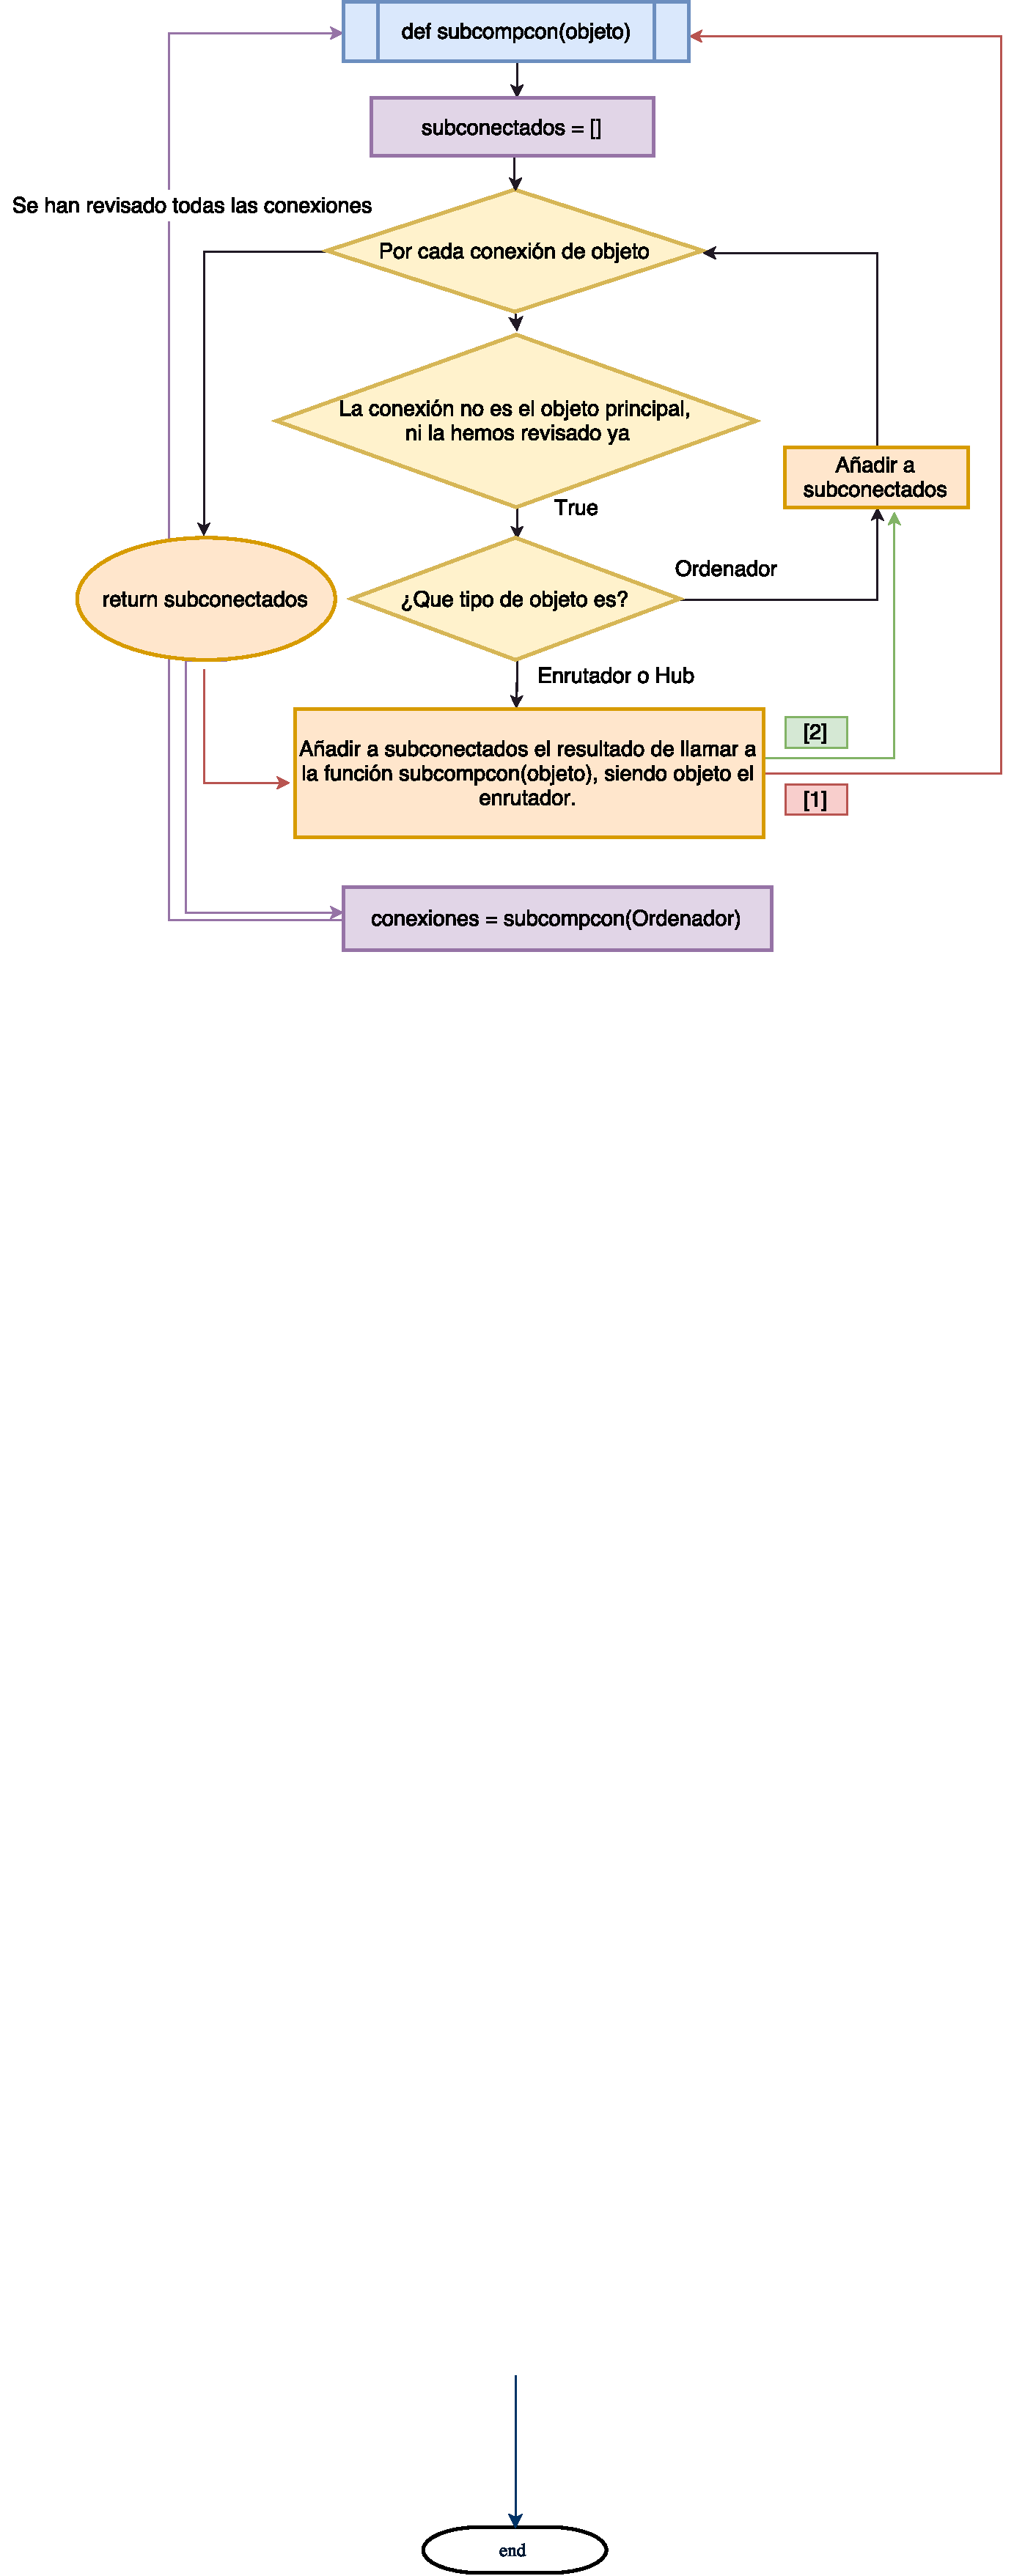
\includegraphics[width=0.9\textwidth]{Resources/Diagramas/Compcon.pdf}
%\caption[Diagrama de flujo de la función compcon]{Diagrama de flujo de la función compcon. Entra en un bucle al volver a llamar a la función de forma recursiva.}
%\end{figure}
%\vspace{\fill}

\subsubsection{mac}
Esta clase es la que crea los objetos que serán una dirección MAC. Transcurre de la línea 1024 a la 1059 y contiene varias funciones técnicas, pero la única importante es \function{genmac}, encargada de generar una dirección MAC aleatoria de 48 bits de longitud.
\subsubsection{Port y w\char`_switch\char`_table}
\class{Port} es una clase que usan los conmutadores y concentradores. Simula un puerto de red. Tan sólo posee cuatro funciones: \function{\char`_\char`_init\char`_\char`_}, que es la que se usa al crear el objeto; \function{connect}, para conectar un objeto al puerto; \function{disconnect}, para desconectarlo y \function{is\char`_available}, para saber si el puerto está disponible u ocupado. \texttt{1080:1099}

La clase \class{w\char`_switch\char`_table} es la encargada de la ventana de visualización de la tabla de enrutamiento del Switch. \texttt{1101:1160}

\subsubsection{Clases de paquetes de red}
Ocupan entre el 25\% y el 30\% del código. Son clases como \class{packet} (la clase base), \class{eth} (paquete con \textit{frame} aplicado, \class{icmp} (paquete con ICMP) y la última clase \class{Ping}, que hereda de \class{icmp} y se encarga de crear un paquete de red, bit a bit, dados una dirección IP de destino y de origen.
Entre todas estas clases debemos destacar dos funciones:
\begin{itemize}
\item \function{animate} es una función que poseen todos los tipos de paquetes de red y se encarga de poner un paquete de red en la interfaz, y de que este se mueva. Para ello, hace una combinación de dos movimientos, uno en el eje x y otro en el eje y, la longitud que debe de moverse en total la divide entre el número total de fotogramas y así consigue la distancia que debe moverse cada fotograma. Cuenta dentro con una subfunción, \function{iteration}, que se encarga de poner la imagen cada fotograma en su sitio y eliminar la imagen del fotograma anterior. Esta función ha sido posible gracias a los conocimientos sobre vectores adquiridos durante primero de 
Bachillerato.\texttt{1627:1717}
\item \function{create} es una función propiedad de \class{Ping}, que dadas una dirección IP de destino y origen, crea un paquete de red, bit a bit, basado en el modelo real de paquetes de Ping inspeccionado por Wireshark, y confirmado en libros de teoría. Es una función que, aunque parezca sencilla, fueron bastantes horas de trabajo, pues es bastante complejo tratar con bits.
\end{itemize}
\inputminted[firstline=1782, lastline=1818, baselinestretch=1, fontsize=\scriptsize, linenos, breaklines]{python}{Codigo/invproy/main.py}

\subsection{Dispositivos}
Existen cuatro tipos dispositivos: los Computadores, que tienen la mayor programación; los Switches, que se encargan de manejar los paquetes de red; los Hubs, que son como los Switches, pero reenvían los paquetes por todos sus puertos y los Routers, que tan sólo existen de forma visual, pero no tienen ninguna función de momento. Por lo que sólo vamos a hablar de los Switches y los Ordenadores. Para cambiar los parámetros hay que hacer click derecho en el dispositivo al que se le deseen cambiar los parámetros y luego en la entrada de `Editar objeto'. A lo que aparecerá una ventana como la de Fig. \ref{fig:editwindow} en la que se podrán cambiar parámetros como el nombre, la dirección MAC o la dirección IP.

Los ordenadores tienen una función especial que es la de crear y enviar los paquetes de red. Para ello, en el menú emergente que aparece al hacer click derecho en el objeto, hacemos click en la entrada de `Ping'. Para que el paquete llegue al otro computador, ambos deben tener una dirección IP, y estar conectados a la misma red. Se introduce la dirección IP del dispositivo y se pulsa en el botón de `Ping!' (Ver Fig. \ref{fig:pingwindow} y Fig. \ref{fig:pingwindow2}). A continuación veremos el paquete de red buscando su objetivo, la primera vez no irá directamente, ya que los Switches están aún aprendiendo el camino, pero el paquete de vuelta y todos los siguientes paquetes seguirán la misma ruta (Ver Fig. \ref{fig:samplenet}). El ordenador crea un paquete de red usando los protocolos de Ethernet (IEEE 802.11), TCP, IPv4 e ICMP. La función que se encarga de esto es \function{create}.

Los Switches se encargan de redireccionar los paquetes de red. La primera vez que les llega un paquete, al no saber la ubicación física del destino, siguen este algoritmo:
\inputminted[firstline=1268, lastline=1296,baselinestretch=1,
	fontsize=\scriptsize,
	linenos,
	breaklines]{python}{Codigo/invproy/main.py}
Este algoritmo esta basado en el que usan los conmutadores reales y, traducido a lenguaje humano, vendría a ser:
\begin{easylist}[itemize]
\ListProperties(Style*=,Space*=6pt)
& Si la dirección MAC de destino del paquete recibido se encuentra directamente conectado al Switch y el TTL del paquete es mayor que cero:
&& Enviar el paquete a ese dispositivo.
& Al no cumplirse la condición anterior, si el paquete se encuentra en mi tabla de enrutamiento y el TTL del paquete es mayor que cero:
&& Enviamos el paquete por el puerto al que está asignada la dirección MAC en la tabla.
& Al no cumplirse las condiciones anteriores, si hay un Switch en mis conexiones y el TTL del paquete es mayor a 0:
&& Enviar el paquete a uno de los Switches de forma aleatoria.
\end{easylist}

Cuando recibe un paquete, también añade a la \textit{Routing Table} o tabla de enrutación una entrada con la dirección MAC del remitente del paquete y el puerto por el que ha llegado, así cuando le llegue un paquete el router conocerá el puerto por el que enviarlo.
\inputminted[firstline=1231, lastline=1247, baselinestretch=1,fontsize=\scriptsize, linenos,breaklines]{python}{Codigo/invproy/main.py}
Este es el código que cumple esta función. Cada elemento en la tabla tiene un tiempo establecido en el que caduca la entrada. Lo que hace esta parte del código es comprobar si este tiempo ha caducado, actualizar la fecha de caducidad si la dirección MAC ya está en la tabla o añadirlo de nuevo en la tabla si la dirección no está.

\section{Versión actual del programa (0.2.4-alpha)}
\label{01}
En la versión 0.1 se introdujo toda la interfaz, las conexiones, los dispositivos... Pero aún no se podían enviar ni recibir paquetes de red. En la versión 0.2 se introdujo esta posibilidad, junto a otras cosas como el enrutamiento de paquetes. El programa es considerado una versión \textit{alpha}, ya que aún está en desarrollo y no es un programa terminado.

El programa te permite, por el momento, hacer una simulación de red simple. Se podría decir que es una base sobre la que se pueden ir añadiendo más funcionalidades, como el soporte para otros protocolos, o un modo `explicatorio' que enseñe a los alumnos lo que está pasando en la red. En la versión 0.2.3-alpha del programa sólo se ha introducido el ``Ping", es decir, la posibilidad de enviar un paquete de prueba a otro dispositivo de la misma red. También se han introducido algunos cambios en la interfaz, uno de ellos, bastante útil para el aprendizaje: los cuadros de texto en los que se introducen direcciones IP, cambian de color entre rojo, naranja o verde, dependiendo si la IP introducida no es válida, está incompleta o es válida, respectivamente.

\section{Desarrollo del proyecto}
En cuanto al código, a pesar de la gran extensión del programa, han sido escritas muchas más líneas, que han sido en algún momento eliminadas o reemplazadas. El desarrollo del proyecto puede dividirse en 4 fases a lo largo de 3 trimestres.

En la primera fase, de Noviembre a Febrero/Marzo he ido aprendiendo sobre todo de Gtk+, la librería para la interfaz del programa. Al empezar el proyecto mis conocimientos sobre esta librería eran nulos; y sobre Python, el lenguaje de programación, eran demasiado básicos. También aprendí bastante sobre redes informáticas.

En la segunda fase, se fue desarrollando la ``base" del programa, transcurre de Febrero-Marzo a finales de curso. La interfaz, las ideas, las conexiones de los cables... Se construye la versión 0.1, como menciono en \ref{01}. El programa contaba con unas 700 líneas en \texttt{Main.py}

En la tercera fase se desarrolla la gran parte del programa, aquí es cuando llega a las 2000 líneas, sin mencionar los pequeños módulos y otros archivos. Transcurre en verano, entre Junio y mediados de Agosto. Con una media de 200-300 líneas semanales y picos de hasta mil líneas entre el 7 y el 14 de Agosto, ha sido posible cumplir el objetivo de crear un pequeño simulador de redes. Es el desarrollo de la versión 0.2-alpha, ya que el programa sigue en desarrollo de posteriores versiones.

La cuarta fase transcurre solapada con la tercera, comienza en Julio y acaba el día \@date, con la entrega de la memoria del proyecto. Es la fase en la que se desarrolla esta memoria.

He notado bastante la adquisición de experiencia, ya que tardé prácticamente 5-6 meses en hacer las primeras 500 líneas; pero en verano, conforme iba programando más, conseguí llegar a hacer más de 1000 líneas en una semana. También, al leer el código antiguo se notan bastantes errores debidos a la falta de experiencia, que tiene que ser corregidos si aún no se ha hecho.

\subsection{Obstaculos en el desarrollo del proyecto}
Durante el desarrollo del proyecto han surgido bastantes trabas y contratiempos, que he conseguido solucionar. Muchos de ellos surgen por la falta del gran conocimiento técnico necesario para la creación de un software tan específico, han sido muchas horas de mirar la documentación de las librerías \cite{PyGiApi}, y pedir ayuda por foros para intentar solucionar dudas y bugs.

En algunas ocasiones no han sido errores, sino falta de conocimiento para el desarrollo de determinadas funciones lo que ha creado pausas de hasta dos semanas en la acción de escribir el programa. Gracias a comunidades como \textbf{\textit{stackoverflow}} he conseguido solucionar muchas de las dudas y errores básicos del programa.

Otro inconveniente ha sido el tiempo, que no me ha dejado implementar funciones útiles, como un visor de paquetes de red, más protocolos, o interconexión de redes.

\newpage
\section{Conclusión}
Lo más difícil fue empezar. El tratar de aprender tanta información de golpe de forma autodidacta. Aunque ya supiese un poco sobre programación en Python, no tenía casi experiencia, aprender a usar la librería de Gtk+, aprender sobre redes, aprender sobre un uso más extenso de GNU/Linux, aprender sobre \LaTeX , etc. fue bastante cansado. pero eso es lo mejor, todo lo que he aprendido y, sobre todo, la experiencia que he adquirido en el campo de la programación.

A la hora de programar, al principio el ritmo era muy lento, de unas 200 líneas al mes, con pausas de semanas para solucionar problemas y errores. Poco a poco se fue acelerando hasta llegar a finales de Julio, donde hacía más de 100 líneas diarias. Aprendiendo en el proceso el uso de clases y decoradores.

Pese a que es verdad que falta incluir más protocolos y algunas funcionalidades bastante básicas (como mover objetos), estoy bastante satisfecho con la versión actual del programa, que se ha realizado con bastante poco tiempo, ya que tiene las bases, y creo que añadir un nuevo protocolo, o una nueva funcionalidad no serían más que unas horas delante de la pantalla y el teclado del ordenador.

Resumiendo:
\begin{easylist}[itemize]
\ListProperties(Style*=\color{chaptercolour}$\bullet$\hspace*{10pt}, Space*=-5pt, Space=0pt)
& Se ha creado un simulador de redes escrito en Python que demuestra el uso de Ping's y enrutamiento de paquetes
& Con el programa actual, es fácil añadir nuevos paquetes, dispositivos o funcionalidades, entre otras cosas
& Se ha desarrollado íntegramente con software libre
& Tiene uso didáctico en 4º de la ESO, 1º y 2º de Bachillerato, pues se incluye `Redes informáticas' en el temario de Informática y TICO, además de `Programación'
& Los alumnos pueden modificar y ampliar el programa, para toda la comunidad educativa, en GitHub
\end{easylist}

\glsaddall
\renewcommand{\glsnamefont}[1]{\makefirstuc{#1}}
\renewglossarystyle{mcolindex}{%
  \setglossarystyle{index}%
  \renewenvironment{theglossary}%
    {%
    \setlength{\columnsep}{30pt}
     \begin{multicols}{\glsmcols}
     \setlength{\parindent}{0pt}%
     \setlength{\parskip}{0pt}%
     \renewcommand\item{\par\hangindent0pt}}%
    {\end{multicols}}%
}

\nocite{*}
%\bibliographystyle{IEEEtranN}
\printbibliography[heading=bibintoc]

\appendix

\chapter{Capturas de pantalla del programa}
\noindent\begin{figure}[H]
\centering
\begin{minipage}[t]{0.4\textwidth}
	%\vtop{
	\centering
	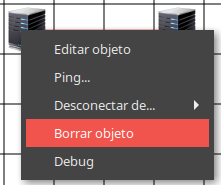
\includegraphics[scale=0.6]{Resources/Screenshots/2016-09-12-172627_1000x700_scrot.png}%}
	\caption{Captura: Click derecho en un computador}
\end{minipage}
\hspace*{0.15\textwidth}
\begin{minipage}[t]{0.4\textwidth}
	%\vtop{
	\centering
	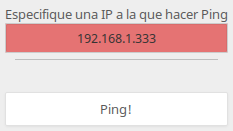
\includegraphics[width=\textwidth]{Resources/Screenshots/2016-09-12-225752_233x131_scrot.png}%}
	\caption[Captura: Ventana para enviar ping.]{Captura: Ventana para enviar ping. Está en rojo porque la IP introducida no es válida.}
	\label{fig:pingwindow}
\end{minipage}

\vspace*{1cm}
\centering
\begin{minipage}[t]{0.4\textwidth}
	\centering
	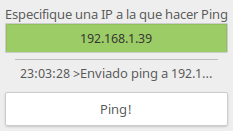
\includegraphics[width=\textwidth]{Resources/Screenshots/2016-09-12-230329_233x131_scrot.png}
	\caption{Captura: Igual que \ref{fig:pingwindow}, pero con una IP válida.}
	\label{fig:pingwindow2}
\end{minipage}
\hspace*{0.15\textwidth}
\begin{minipage}[t]{0.4\textwidth}
	\centering
	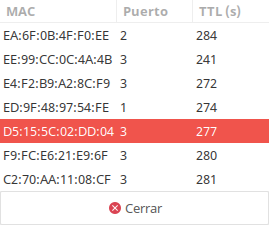
\includegraphics[scale=0.6]{Resources/Screenshots/2016-09-12-230428_269x225_scrot.png}
	\caption{Captura: Ventana con la tabla que poseé el Switch.}
	\label{fig:switchingtable}
\end{minipage}

\vspace*{1cm}
\centering
\begin{minipage}[t]{0.5\textwidth}
	\centering
	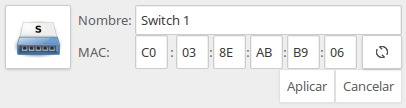
\includegraphics[scale=0.6]{Resources/Screenshots/2016-09-13-200254_406x108_scrot.png}
	\caption{Captura: Ventana de edición de propiedades de objeto.}
	\label{fig:editwindow}
\end{minipage}

\end{figure}
\begin{figure}[H]
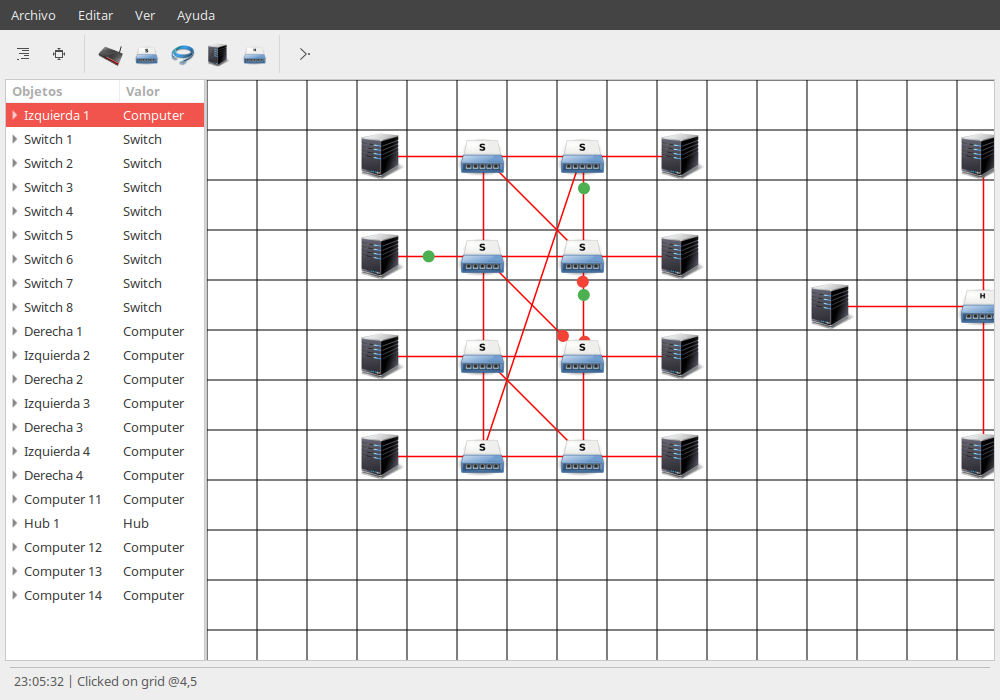
\includegraphics[width=\textwidth]{Resources/Screenshots/2016-09-12-230644_1000x700_scrot.png}
\caption{Captura: Paquetes viajando por una red de ejemplo.}
\label{fig:samplenet}
\end{figure}

%\chapter{Código del programa}
%\begin{listing}
\newcommand{\ipm}[1]{
	\section{#1}
	\inputminted[baselinestretch=1, fontsize=\tiny, linenos, breaklines]{python}{Codigo/#1}
}
\ipm{Main.py}
\ipm{Modules/logmod.py}
\ipm{Modules/save.py}
%\section{Interface2.glade} \inputminted[baselinestretch=1, fontsize=\scriptsize, linenos, breaklines]{XML}{Codigo/Interface2.glade}

%\end{listing}

\newpage
\thispagestyle{empty}
\newgeometry{left=2.5cm, top=1cm, right=2cm, bottom=2cm, headheight=14pt}
\topskip0pt
\vspace*{2cm}
\doclicenseThis

\noindent
\begin{minipage}{0.7\textwidth}
\noindent El software InvProy está realizado bajo la licencia \href{https://www.gnu.org/licenses/quick-guide-gplv3.html}{GNU GPLv3}
\end{minipage}
\hspace*{\fill}
\begin{minipage}{0.3\textwidth}
\hspace*{\fill}

\includegraphics[height=1.4cm]{Resources/gplv3-127x51.png}
\end{minipage}

\noindent
Encontrará una copia del código y la licencia en \url{https://github.com/daviddavo/InvProy} \\
Encontrará una copia de este documento en \url{https://github.com/daviddavo/InvProy-tex}\\

\centering
InvProy \hspace*{10pt} Copyright \copyright\hspace*{10pt} 2016 \hspace*{15pt} David Davó Laviña \\ \hspace*{15pt} david@ddavo.me \hspace*{10pt} \url{http://ddavo.me}

\vspace{0.7cm}
\noindent\centering
\begin{minipage}{13cm}
\centering Podrá encontrar una copia digital del documento, el software, las licencias y los recursos usados en el CD adjunto.
\end{minipage}

\vspace*{1cm}
\centering\framebox[12.5cm]{
%\begin{tabularx}{1cm}{|c|} 
%\rowcolor{chaptercolour} \\
%\rowcolor{sectioncolour} \\
%\rowcolor{subsectioncolour} \\
%\rowcolor{subsubsectioncolour} \\
%\rowcolor{header} \\
%\end{tabularx}
\raisebox{0pt}[12.5cm][0pt]{
}} %\par
%\vspace*{\fill}

%\restoregeometry
\end{document}
